% fig_67_coverage.tex
% TR-32: Coverage map on (alpha, k_ibr) plane for 67N+67Q combined scheme
%
% Same axes as TR-29 coverage map: alpha [0,1] x k_ibr [0.06, 0.20]
% Coordinate scaling: x = alpha*10, y = (k_ibr-0.06)/0.14*7
%
% 67N coverage: ALL regions (I0 from network, indep. of k_ibr)
%   colour: green!35 everywhere
%
% 67Q coverage: k_ibr >= I_min_67 = 0.04 pu
%   Since k_ibr range shown is [0.06, 0.20], ALL shown region has k_ibr >= 0.04
%   colour: green!55 (darker, on top of 67N)
%
% Key boundaries (from TR-29):
%   k_ibr = 0.10: 21 I_min threshold (horizontal, red solid)
%   alpha = 0.80: Zone 1 boundary (dash-dot grey)
%
% New boundary for 67Q (not shown in TR-29):
%   k_ibr = 0.04 (67Q lower limit) — below the displayed range

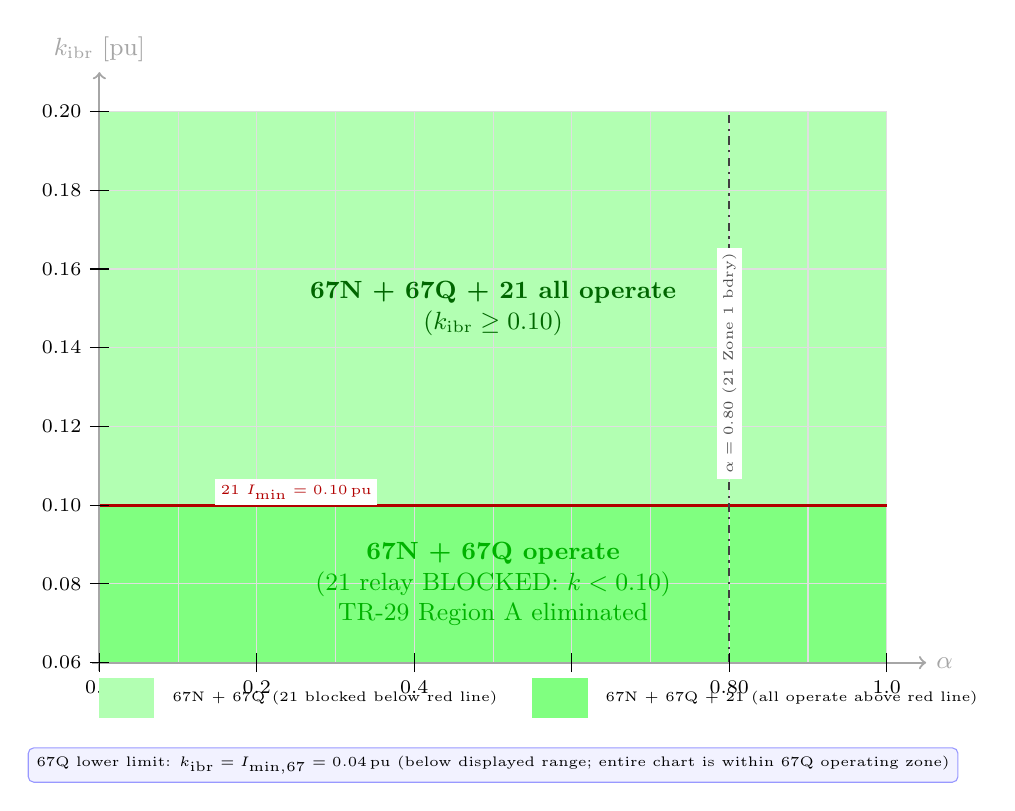
\begin{tikzpicture}[
  every node/.style = {font=\scriptsize},
]

% ── Fill: both 67N and 67Q operate everywhere in the displayed range ──────
\fill[green!30] (0,0) rectangle (10,7);

% ── Highlight: zone where 21 is blocked but 67N/67Q operates ─────────────
% k_ibr < 0.10 → y < (0.10-0.06)/0.14*7 = 2.0
\fill[green!50] (0,0) rectangle (10, 2.0);

% ── Grid ──────────────────────────────────────────────────────────────────
\draw[gray!25, step=1.0] (0,0) grid (10,7);

% ── Boundary lines ────────────────────────────────────────────────────────
% k_ibr = 0.10 (21 I_min threshold)
\draw[red!70!black, very thick] (0, 2.0) -- (10, 2.0);
% alpha = 0.80 (Zone 1 boundary)
\draw[gray!50!black, thick, dash dot] (8.0, 0) -- (8.0, 7.0);

% ── Axes ──────────────────────────────────────────────────────────────────
\draw[->, thick, gray!70] (-0.1, 0) -- (10.5, 0)
  node[right, font=\small] {$\alpha$};
\draw[->, thick, gray!70] (0, -0.1) -- (0, 7.5)
  node[above, font=\small] {$k_\mathrm{ibr}$ [pu]};

\foreach \a/\x in {0.0/0, 0.2/2, 0.4/4, 0.6/6, 0.80/8, 1.0/10} {
  \draw (\x, -0.12) -- (\x, 0.12);
  \node[below=3pt] at (\x, 0) {\a};
}
\foreach \k/\y in {0.06/0, 0.08/1, 0.10/2, 0.12/3, 0.14/4, 0.16/5, 0.18/6, 0.20/7} {
  \draw (-0.12, \y) -- (0.12, \y);
  \node[left=3pt] at (0, \y) {\k};
}

% ── Region labels ─────────────────────────────────────────────────────────
% Lower region (21 blocked, but 67N+67Q OK)
\node[green!70!black, font=\small, align=center] at (5.0, 1.0)
  {\textbf{67N + 67Q operate}\\(21 relay BLOCKED: $k<0.10$)\\TR-29 Region~A eliminated};

% Upper region (all elements operate)
\node[green!40!black, font=\small, align=center] at (5.0, 4.5)
  {\textbf{67N + 67Q + 21 all operate}\\($k_\mathrm{ibr} \geq 0.10$)};

% ── Boundary annotations ──────────────────────────────────────────────────
\node[red!70!black, fill=white, inner sep=2pt, font=\tiny]
  at (2.5, 2.0) [above] {21 $I_\mathrm{min}=0.10$\,pu};

\node[gray!60!black, fill=white, inner sep=2pt, font=\tiny, rotate=90]
  at (8.0, 3.8) {$\alpha=0.80$ (21 Zone~1 bdry)};

% ── 67Q lower limit note (below the chart) ────────────────────────────────
\node[font=\tiny, align=center, draw=blue!40, fill=blue!5,
      rounded corners=2pt, inner sep=3pt]
  at (5.0, -1.3)
  {67Q lower limit: $k_\mathrm{ibr} = I_\mathrm{min,67} = 0.04$\,pu
   (below displayed range; entire chart is within 67Q operating zone)};

% ── Legend ────────────────────────────────────────────────────────────────
\fill[green!30] (0.0, -0.7) rectangle (0.7, -0.2);
\node[right=3pt, font=\tiny] at (0.7, -0.45)
  {67N + 67Q (21 blocked below red line)};

\fill[green!50] (5.5, -0.7) rectangle (6.2, -0.2);
\node[right=3pt, font=\tiny] at (6.2, -0.45)
  {67N + 67Q + 21 (all operate above red line)};

\end{tikzpicture}
